\documentclass[]{article}
\usepackage{lmodern}
\usepackage{amssymb,amsmath}
\usepackage{ifxetex,ifluatex}
\usepackage{fixltx2e} % provides \textsubscript
\ifnum 0\ifxetex 1\fi\ifluatex 1\fi=0 % if pdftex
  \usepackage[T1]{fontenc}
  \usepackage[utf8]{inputenc}
\else % if luatex or xelatex
  \ifxetex
    \usepackage{mathspec}
  \else
    \usepackage{fontspec}
  \fi
  \defaultfontfeatures{Ligatures=TeX,Scale=MatchLowercase}
\fi
% use upquote if available, for straight quotes in verbatim environments
\IfFileExists{upquote.sty}{\usepackage{upquote}}{}
% use microtype if available
\IfFileExists{microtype.sty}{%
\usepackage{microtype}
\UseMicrotypeSet[protrusion]{basicmath} % disable protrusion for tt fonts
}{}
\usepackage[margin=1in]{geometry}
\usepackage{hyperref}
\hypersetup{unicode=true,
            pdftitle={The Relationship Between Exercise Time and Weight Loss},
            pdfauthor={Bilal Mozaffar, Risheng Li, Thomas Janes},
            pdfborder={0 0 0},
            breaklinks=true}
\urlstyle{same}  % don't use monospace font for urls
\usepackage{graphicx,grffile}
\makeatletter
\def\maxwidth{\ifdim\Gin@nat@width>\linewidth\linewidth\else\Gin@nat@width\fi}
\def\maxheight{\ifdim\Gin@nat@height>\textheight\textheight\else\Gin@nat@height\fi}
\makeatother
% Scale images if necessary, so that they will not overflow the page
% margins by default, and it is still possible to overwrite the defaults
% using explicit options in \includegraphics[width, height, ...]{}
\setkeys{Gin}{width=\maxwidth,height=\maxheight,keepaspectratio}
\IfFileExists{parskip.sty}{%
\usepackage{parskip}
}{% else
\setlength{\parindent}{0pt}
\setlength{\parskip}{6pt plus 2pt minus 1pt}
}
\setlength{\emergencystretch}{3em}  % prevent overfull lines
\providecommand{\tightlist}{%
  \setlength{\itemsep}{0pt}\setlength{\parskip}{0pt}}
\setcounter{secnumdepth}{0}
% Redefines (sub)paragraphs to behave more like sections
\ifx\paragraph\undefined\else
\let\oldparagraph\paragraph
\renewcommand{\paragraph}[1]{\oldparagraph{#1}\mbox{}}
\fi
\ifx\subparagraph\undefined\else
\let\oldsubparagraph\subparagraph
\renewcommand{\subparagraph}[1]{\oldsubparagraph{#1}\mbox{}}
\fi

%%% Use protect on footnotes to avoid problems with footnotes in titles
\let\rmarkdownfootnote\footnote%
\def\footnote{\protect\rmarkdownfootnote}

%%% Change title format to be more compact
\usepackage{titling}

% Create subtitle command for use in maketitle
\providecommand{\subtitle}[1]{
  \posttitle{
    \begin{center}\large#1\end{center}
    }
}

\setlength{\droptitle}{-2em}

  \title{The Relationship Between Exercise Time and Weight Loss}
    \pretitle{\vspace{\droptitle}\centering\huge}
  \posttitle{\par}
    \author{Bilal Mozaffar, Risheng Li, Thomas Janes}
    \preauthor{\centering\large\emph}
  \postauthor{\par}
      \predate{\centering\large\emph}
  \postdate{\par}
    \date{2/6/2021}

\usepackage{booktabs}
\usepackage{longtable}
\usepackage{array}
\usepackage{multirow}
\usepackage{wrapfig}
\usepackage{float}
\usepackage{colortbl}
\usepackage{pdflscape}
\usepackage{tabu}
\usepackage{threeparttable}
\usepackage{threeparttablex}
\usepackage[normalem]{ulem}
\usepackage{makecell}
\usepackage{xcolor}

\begin{document}
\maketitle

\hypertarget{abstract}{%
\section{Abstract}\label{abstract}}

The purpose of this data analysis is to determine whether and how total
metabolic minutes and employee shift time affect weight gain. The data
are from a survey administered to call center employees from a start
time for call center workers. The survey covers a time period of eight
months. We will apply different methods to limit the effect of missing
data and to create statistical models to determine the effects of
certain variables. We will create \emph{insert models here, describing
response variable for each}

\hypertarget{introduction}{%
\section{Introduction}\label{introduction}}

In the age of computing, more people continue to find jobs that require
them to sit all day. Physical activity at the workplace is not as common
as it once was, which can potentially lead to unwanted health
consequences. It is important to deduce which factors related to the
workplace may have a role in influencing health metrics such as weight
gain. Doing so may help prevent health issues among employees in the
long-run.

Our goal is to detect whether factors, particularly total metabolic
minutes, a measure of the intensity and duration of a person's physical
activity in minutes per week, and shift time, affect weight gain for
employees of a call center. We will create \emph{descriptive statistics
and plots} to visualize these relationships in order to generate models
that could answer these questions. The models will be \emph{insert
models and response variables}. This report details our analytical
decisions and insights.

\hypertarget{the-data}{%
\section{The Data}\label{the-data}}

The data used in this analysis were provided by the call center. The
data consist of 392 observations and 83 variables, including 12
variables of interest. We remove 40 empty observations. Total metabolic
minutes is a critical variable in this analysis, and some observations
are missing this variable value. However, we calculate and replace many
of these missing values using the following equation:

\(Total\:Metabolic\:Minutes\:=\:8\:*Vigorous\:Exercise\:Time\:+\:4\:*\:Moderate\:Exercise\:Time\:+\:3.3\:*\:Walking\:Exercise\:Time\)

For the numerical pounds gained variable, there are many N/A values. For
observations that have a binary weight gain value of ``No,'' we change
the numerical pounds gained value to 0 to indicate that this observation
did not gain weight. Because the numerical pounds gained variable cannot
be calculated using a transformation of other variables, we remove
certain observations that have missing pounds gained and weight gain
variables.

We calculate and input values for beginning weight by subracting pounds
gained from body weight. We also calculate beginning BMI using a
transformation of beginning weight and height:

\(Beginning\:BMI\:=\:730\:*(Beginning\:Weight\:/\:(\:Height\:^2))\)

\hypertarget{exploratory-data-analysis}{%
\section{Exploratory Data Analysis}\label{exploratory-data-analysis}}

In order to see whether certain covariates are correlated, We create
pairs plots to observe basic trends. We look at continuous numerical
variables, because their trends are more meaningful than factor
variables. We also look at the shift variable, because it is numerically
ranked and is very relevant to this study's primary purpose.

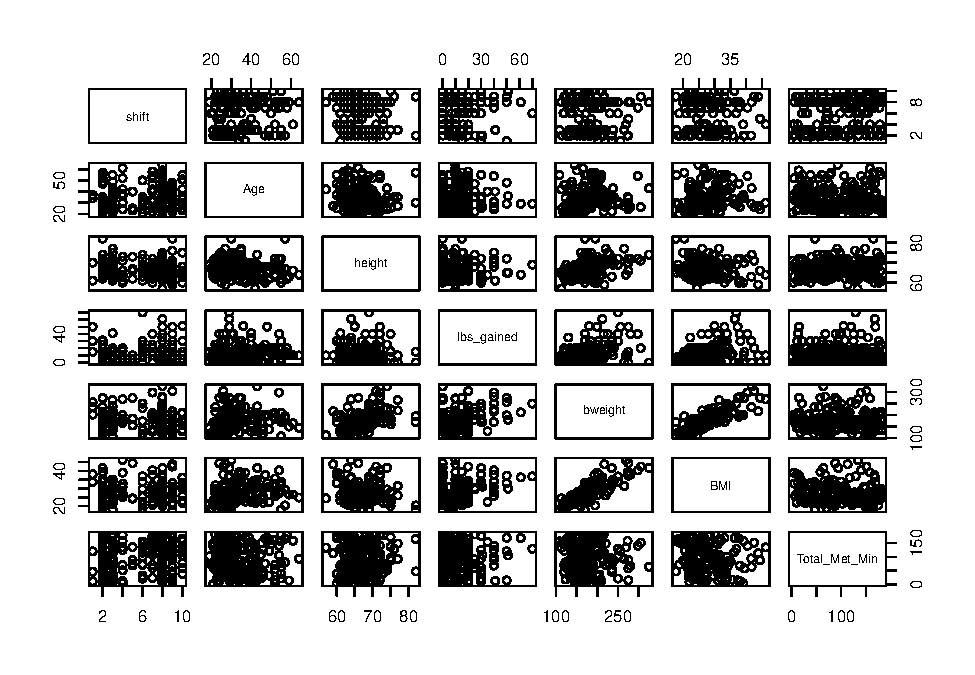
\includegraphics{Practicum-1-Technical-Report-v2_files/figure-latex/Pairs Plots-1.pdf}

As expected, body weight and BMI have a strict positive correlation, as
BMI is linearly dependent upon body weight. Height also has a positive
relationship with lbs\_gained, as intuitively expected. Besides these
and other expected relationships, there are not many easily discernible
correlations. Specifically, neither shift nor total metabolic minutes
has an evident relationship with pounds gained.

We now will observe density plots of certain variables to see whether
any transformations will be beneficial.

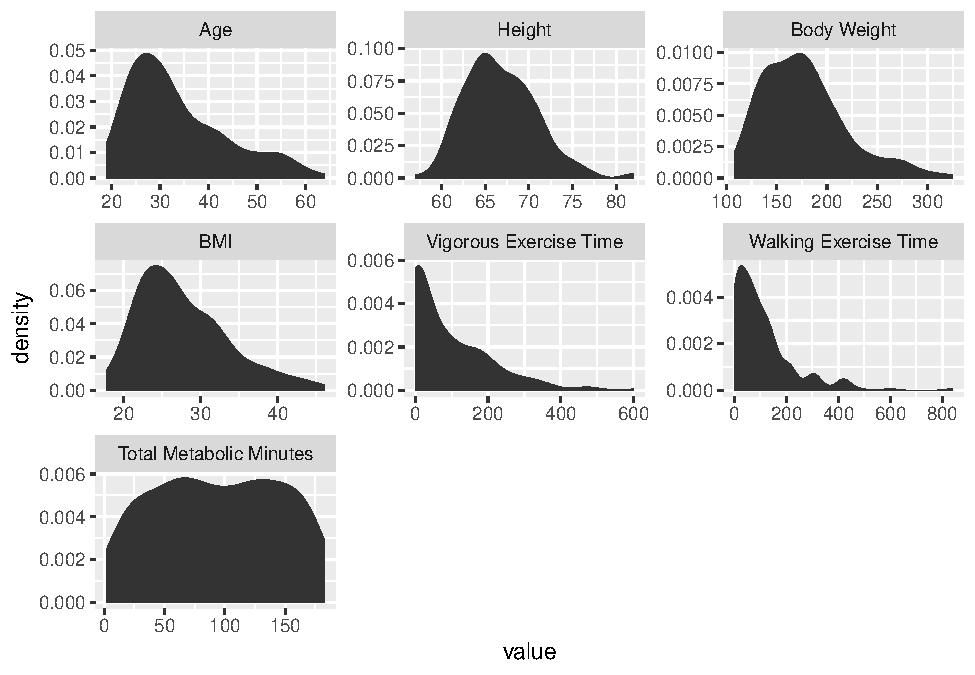
\includegraphics{Practicum-1-Technical-Report-v2_files/figure-latex/unnamed-chunk-2-1.pdf}

Although several variables are right-skewed, We see that Age and BMI are
not only right-skewed but also have no zero values, so we will do log
transformations on these variables. This will aid in the creation of the
linear models by making the assumptions of normality more realistic.

We will group different shift values together as follows:

Early morning: shift beginning from 7 to 9am

Late morning: shift beginning from 10 to 11am

Afternoon: shift beginning from 12 to 2pm

Other: other

N/A: NA

To analyze potential effects of shift and total metabolic minutes
simultaneously, we look at a scatterplot with total metabolic minutes as
the independent variable and pounds gained as the response variable,
with observations colored by shift category.

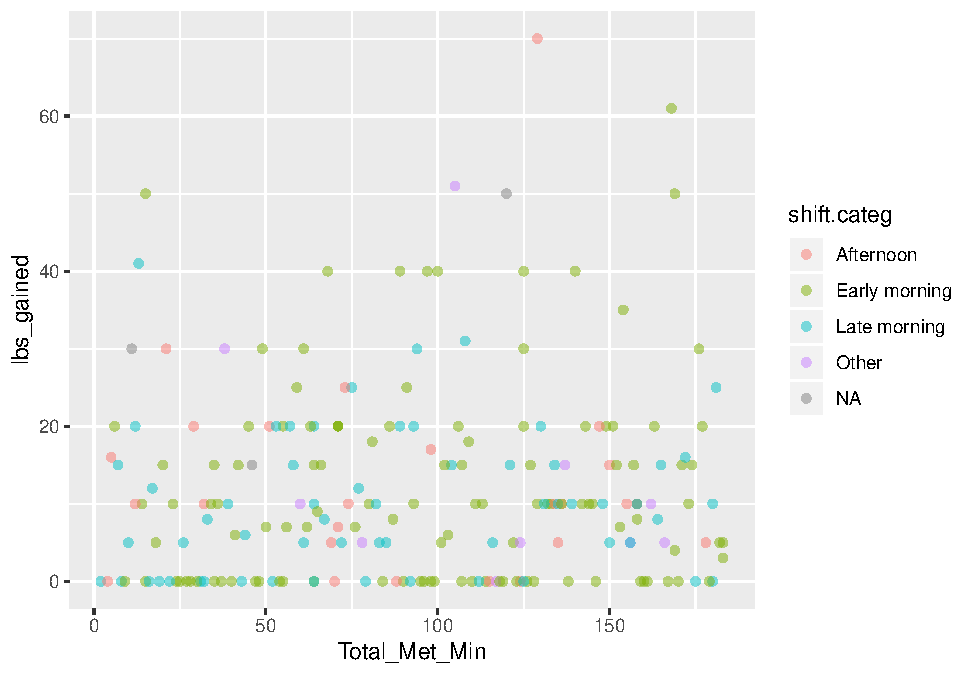
\includegraphics{Practicum-1-Technical-Report-v2_files/figure-latex/unnamed-chunk-5-1.pdf}

The response variable, pounds appears to be evenly scattered among all
values of the independent variable, total metabolic minutes. This, like
the earlier pairs plots, suggests that total metabolic minutes may not
strongly influence pounds gained. Moreover, the different colors on the
plot do not seem to follow any particular pattern or trend, suggesting,
like the earlier pairs plots, that shift may not be very relevant in
predicting pounds gained either.

\hypertarget{modeling}{%
\section{Modeling}\label{modeling}}

We want to create two different models. One model will be a binary
logistic regression model, which will have a Yes/No response variable of
weight gain. The second model will be a simple linear regression model,
with the numerical pounds gained variable as the response. There are
benefits and drawbacks to each model. The generalized linear model (GLM)
will have more realistic interpretations for observations that had
missing numerical pounds gained values, whiole the simple linear
regression model will be better at quantifying the effects of certain
covariates.

\hypertarget{model-1-generalized-linear-model-glm}{%
\subsection{Model 1: Generalized Linear Model
(GLM)}\label{model-1-generalized-linear-model-glm}}

By turning weight gain into a dummy variable and performing a logistic
regression, we can see whether other variables have influence on weight
gain. First, we factor the two categorical variables and build a model
with variables including shift category, gender, age, height, and
beginning BMI and total metabolic minutes. Because the change in BMI is
very minimal for the vast majority of observations, we decide to use the
beginning BMI as one of the regressors.

We create two GLMs, one that includes shift category as a predictor and
one that omits shift category. We will then perform a Chi-squared test
to see which of the two models is preferred.

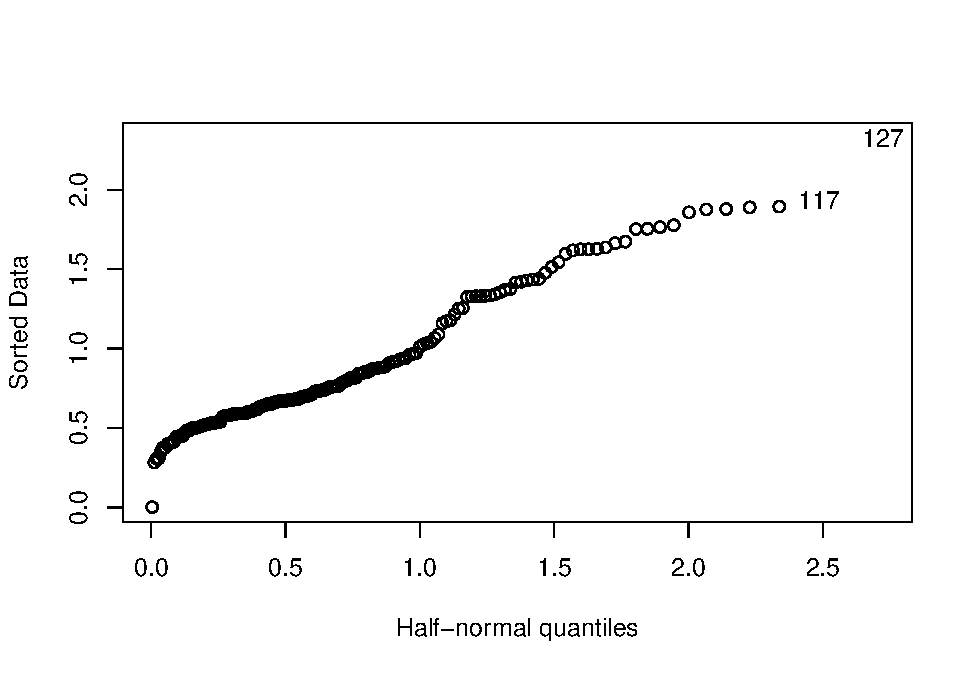
\includegraphics{Practicum-1-Technical-Report-v2_files/figure-latex/unnamed-chunk-6-1.pdf}

The half normal plot for the GLM that includes shift category shows that
there are no obvious outliers in the model.

We now look at the significance of variables in this model.

\begin{verbatim}
##                           Coefficient Estimate P-value
## Shift time: Early Morning -0.7879               0.2947
## Shift time: Late morning  -0.3766               0.6314
## Shift time: Afternoon     -1.0870               0.8240
## Gender: Female             1.6100               0.2903
## Gender: Male               0.7895               0.6010
## Beginning BMI             -0.0670               0.0205
## Total Metabolic Minutes   -0.0001               0.0890
\end{verbatim}

In the model that includes shift category as a predictor of the binary
weight gain response, only beginning BMI appears to be significantly
indicative using a confidence level of 95\%. None of the shift
categories seem to influence weight gain.

We now look at the significance of variables in a new GLM that does
\emph{not} include shift category.

\begin{verbatim}
##                           Coefficient Estimate P-value
## Shift time: Early Morning -0.7879               0.2947
## Shift time: Late morning  -0.3766               0.6314
## Shift time: Afternoon     -1.0870               0.8240
## Gender: Female             1.6100               0.2903
## Gender: Male               0.7895               0.6010
## Beginning BMI             -0.0670               0.0205
## Total Metabolic Minutes   -0.0001               0.0890
\end{verbatim}

With the new model not including shift category, beginning BMI again is
the only significant predictor of the binary weight gain response.

We perform a Chi-sqaure test to test whether the model that contains
shift category is preferred over the model without shift category. The
null hypothesis is that the reduced model, i.e.: the model without shift
category, is a superior model, and the alternative hypothesis is that
the model without shift category is not a weaker model. In order to
compare two models, we omit the NA values in the dataset to make sure
the number of cases used in each model is the same.

\begin{verbatim}
##          P-Value
## Chi-test 0.635
\end{verbatim}

We get a P-value of 0.635, which is very large given a confidence level
of 95\%. Therefore, we fail to reject the null hypothesis that the
reduced model is superior. In other words, there is not enough evidence
to favor the model that includes shift category. It is evident that
shift is not significantly indicative of weight gain.

\hypertarget{model-2-simple-linear-regression-slr}{%
\subsection{Model 2: Simple Linear Regression
(SLR)}\label{model-2-simple-linear-regression-slr}}

Since the initial model shows that Total\_Met\_Min is a significant
variable, we performed another analysis, using a forward stepwise
selection to select the model with the most appropriate variables that
produces the lowest AIC. The selected variables are exactly the same as
our previous analysis, which are gender, Beg\_BMI and Total\_Met\_Min,
which reassures that total metabolic minutes do have an effect on weight
gain and shift does not have an effect on weightgain.

\hypertarget{the-relationship-between-total-metabolic-minutes-and-weight-gain}{%
\subsection{The Relationship Between Total Metabolic Minutes and Weight
Gain}\label{the-relationship-between-total-metabolic-minutes-and-weight-gain}}

Using various methods of analysis, we found that total metabolic minutes
is a significant variable. The initial model demonstrated that there is
a negative relationship between total metabolic minutes and weight gain,
and this was corroborated by the subsequent forward stepwise model.

\hypertarget{the-relationship-between-shift-time-and-weight-gain}{%
\subsection{The Relationship Between Shift Time and Weight
Gain}\label{the-relationship-between-shift-time-and-weight-gain}}

It does not appear that shift has significant impact on weight gain.
From the Chi-square test, we found that the model without shift performs
better than the model with shift. As mentioned, we failed to reject the
null hypothesis that the reduced model is better, so we do not find it
beneficial to include shift in our final model to predict weight gain.

\hypertarget{discussion-and-conclusion}{%
\section{Discussion and Conclusion}\label{discussion-and-conclusion}}

ascertain

Our initial goal was to see whether shift and total metabolic minutes
have an impact on weight gain. Multiple forms of analysis indicate that
shift is not a relevant factor in determining weight gain, while total
metabolic minutes is. Total metabolic minutes has a slightly adverse
relationship to weight gain. We conducted further analysis to go beyond
the requested covariate relationships. For a final model selection,
gender, Beg\_BMI, and Total\_Met\_Min appear to be the most signficant
and useful predictors of weight gain.


\end{document}
